\documentclass[12pt,journal,compsoc]{D:/Магистратура/English/bare_conf/IEEEtran}
\newcommand\MYhyperrefoptions{
pdfpagemode={UseOutlines},plainpages=false,pdfpagelabels=true,
colorlinks=true,linkcolor={black},citecolor={black},urlcolor={black},
pdftitle={Working with attached to repair documents in the system of automatic registration of repairs},
pdfsubject={Typesetting},
pdfauthor={Arseny Zorin}}
\usepackage{graphicx}
\graphicspath{{D:/Магистратура/English/bare_conf/}}

\begin{document}
\title{Working with attached to repair documents in the system of automatic registration of repairs}

\author{Arseny~Zorin}
\maketitle

\IEEEpeerreviewmaketitle



\section{Introduction}
\IEEEPARstart{S}ince the appearance of computers, progress isn't standing still. Technology has enormously improved in last decade. Among trends that appear one can find an ambient wireless Internet access to printing prosthesis on 3D printers or cloud storages. The latter became storage de-facto standard for past few years. It is used not only for private, but also for corporates document storing and data archiving.

The object of research is the authorized service center (ASC) that provides warranty and paid repair of household appliances. There are four branches situated in different parts of the city that take equipment for repair. Each repair operation performed by ASC produces an number of attached documents, their names equal to the ticket number:
\begin{itemize}
\item A photo of schild from back of equipment. This file is stored in a common folder for schilds' photos of this manufacturer.
\item A scanned warranty ticket. This file is stored in a common folder for scanned documents of this manufacturer.
\item An outbound repair receipt. Produced in case the repair was carried out at the client's residence. This file is stored in a common folder of outbound repairs for this manufacturer.
\item Various acts provided to a client including a technical condition act, a non-repairable act, a replacing device act.
\end{itemize}

All document folders are stored at branches offices and at the head office server. Data is transmitted between branches and the head office through FTP protocol.

This work was motivated by a need for modernization of tools for documents storage and transmition. The software programming language was C\# instead of VBA. For scanning documents and making photo of them new libraries will be used. All documents storage were moved to the cloud. Data will be stored and treated at the distributed servers in network. While using cloud storages, users have a possibility to access the data from different places and from different devices which have an Internet access. Also cloud storage can prevent losing information in case of failure of a local storage.

\section{Practical implementation}
\subsection{Working with AForge.NET}
\IEEEPARstart{T}aking photo of a schild: after the button pressed, a new window with video player element will open. Stream video from selected web-camera will be played on this element. After the button "Take a snapshot" pressed, there will be capture of the picture from video player element and an obtained picture will be stored in the specified directory in .jpg format. 

The .NET Framework does not support working with web-cameras it means that there is no video playback element. However, there is namespace AForge.Controls with VideoSourcePlayer element in AForge.NET. This element was created only for using in Windows Forms software. The decision of developing software with using WPF was taken and there are few methods of solution:
\begin{itemize}
\item The creation of a hybrid application. In addition to the WPF window, there will be one Windows Forms window.
\item Using a WindowsFormsHost element. This element allows to place Windows Forms element on WPF page.
\end{itemize}

The latter variant was selected. Forits realization we have to add: System.Windows.Forms.Integration and AForge.Controls namespaces, WindowsFormsHost element and VideoSourcePlayer inside it (Fig. 1).
\begin{figure}[h]
\centering
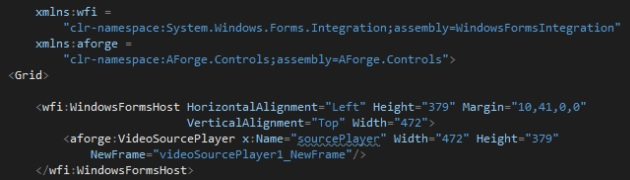
\includegraphics[width=0.5\textwidth]{1}
\centering
\caption{Adding namespces and elements}
\end{figure}

In addition to the playback element we have to add elements for interaction with VideoSourcePlayer element:
\begin{itemize}
\item "Take a snapshot" button
\item List of playback sources
\end{itemize}
After addition of all elements, the window in "Constructor" mode will looks like on fig. 2.
\begin{figure}[h]
\centering
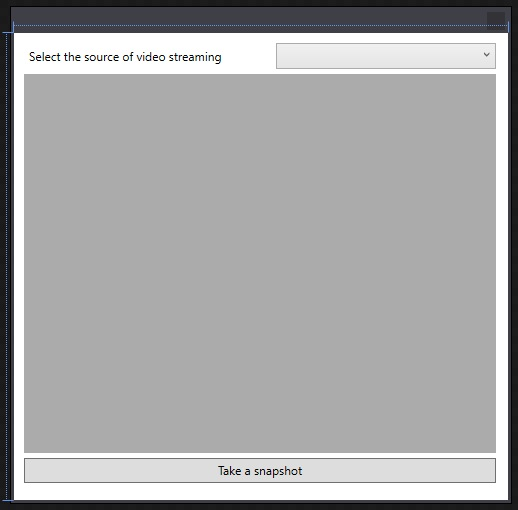
\includegraphics[width=0.5\textwidth]{2}
\centering
\caption{Window view in the constructor mode}
\end{figure}

There is the AForge.Video.DirectShow. VideoCaptureDevice class for capturing video from an input-output (I/O) device. It is necessary to set device's moniker (the name of a cpecific instance of an object. It is a COM-object that has its own way to create and maintain a special interface - IMoniker), which will capture the picture. In addition, we have to add event handler NewFrame. Every time new frame will be received, this event will raise. Received frame sends to the handler in the Bitmap format. It can be processed and stored in the specified format in the right place.

The list will be filled with names of all connected I/O devices and the default device will be the first in the list.

The event comboBoxSources\_SelectedIndexChanged rises after changing selection of source. It stops streaming from previous I/O device, set a moniker to the VideoCaptureDevice class of a new selected device and resumes streaming.

Pressing the button "Take a snapshot" changes the value of the take\_pict boolean variable on true. The value of this variable checks in the event raised after receiving of a new frame. If its value equals to true, then received image saves in .jpg format in specified place. In our case - Yandex.Disk.

The method EndOfWork, that stops streaming and frees used resources, is called after after closing the window.

\subsection{Working with TWAIN library}
We need to program a button for documents scanning. There will be selection of data sources after clicking on the button (if there are several connected scanners). After selecting of the source, scanning will start and received file will be stored at the specific folder in .jpeg format. We have to close data source after finishing the scanning.

There are a lot of different methods in the TWAIN library. However, only several of them will be used for completing the task:
\begin{itemize}
\item OpenDataSource() - Opens a data source. Type of return value - bool. Value true if operation is successful, else - false. 
\item SelectDataSource() - Shows dialog window for selecting a data source. Type of return value - bool. Value true if operation is successful, else - false.
\item Property ShowUI - Gets or sets a value indicating wether to show user interface (UI) of TWAIN-source (to speed up value sets as false)
\item Acquire() - Gets an image from a data source. Type of return value - void. 
\item GetImage(int index) - Returns a scanned image. The parameter index - index of return image. Type of return value - System.Drawin.Image. 
\item CloseDataSource() - Closes a data source. Type of return value - bool. Value true if operation is successful, else - false.
\end{itemize}

The platform of developed software was changed to 32-bit(x86). The reason is that 64-bit(x64) platform is not supported with all scanners.

\subsection{Working with Microsoft.Office.Interop}
For beginning the work with Word and Excel documents from Visual Studio, it is necessary to add references into the project: Microsoft.Office.Interop.Word and Microsoft.Office.Interop.Excel. 

\subsubsection{Working with Microsoft.Office.Interop.Word}
The words starting wigth \@ must be replaced with values of table cells during the creation of acts. Application object, which is the parent of all objects, used for working  in the .NET. The work with its methods and properties is available after the reference on this object was received. This object provides a big set of methods and properties that allows to manage the Microsoft Word. 

Particularly all Word functions require an object parameters.


\subsubsection{Working with Microsoft.Office.Interop.Excel}

\subsection{Working with Yandex.Disk}

\section{Conclusion}

\end{document}
